\documentclass[11pt]{article}

\usepackage{my_article_header}
\usepackage{graphicx}
\usepackage{float}
\usepackage{booktabs}
\usepackage{float}
\usepackage{placeins}

\setlength{\parindent}{0pt}
\setlength{\parskip}{0.8em}


\title{Can ChatGPT Forecast Stock Price Movements? Return Predictability and Large Language Models}
\author{Langxuan Pan, Yiguang Zhu}
\date{\today}

\begin{document}

\maketitle

\section{Introduction}

This project investigates whether large language models, specifically ChatGPT, can forecast stock price movements by analyzing firm-level news headlines. The central idea is that news sentiment, as interpreted by a language model, can provide information about future stock returns. By classifying news as positive, neutral, or negative, it is possible to construct long and short portfolios and evaluate whether these signals produce abnormal returns.

The goal of this study is to assess the predictive power of language model-generated sentiment labels in a systematic trading strategy. In particular, the project focuses on constructing a trading strategy using sentiment-labeled news headlines and evaluating the resulting portfolio performance over time.

\section{Data Sources}

The replication project combines multiple datasets to construct the trading strategy.

First, stock return data were obtained from CRSP-based daily equity data. These data provide information on daily stock prices, including opening and closing prices, which are used to compute next-day returns for news events released outside of trading hours.

Second, intraday price data were obtained from the TAQ (Trade and Quote) database. TAQ provides high-frequency transaction and quote information during trading hours. These data are used to calculate intraday returns for news events released during market hours, allowing us to measure the immediate price reaction to news announcements.

Third, news event data were obtained from the RavenPack database, which provides structured information on financial news, including the timestamp of each news release and the associated firm ticker. The timestamps allow us to determine whether a news event occurs during trading hours or outside of trading hours, which determines whether intraday or next-day returns are used.

Finally, the dataset includes sentiment labels generated using a large language model. These labels classify each news headline as either positive (YES), negative (NO), or neutral (UNKNOWN) with respect to expected stock price movements. These classifications are used to construct trading signals for the long-short, long-only, and short-only portfolios.

\section{Data Exploration}

Before constructing the trading strategy, we conduct a brief exploratory analysis of the main datasets used in the replication. The purpose of this section is to illustrate the characteristics of each data source and provide a basic overview of the information contained in the datasets.

\FloatBarrier
Table~\ref{tab:crsp_summary} reports summary statistics of the CRSP daily equity dataset used in the analysis. The table summarizes key variables including daily returns, opening prices, closing prices, trading volume, and market capitalization. The statistics show that daily stock returns are centered around zero, while stock prices and market capitalization vary substantially across firms, reflecting the diversity of firms in the sample.

\begin{table}
\centering
\caption{Summary statistics of CRSP daily stock data used in the replication.}
\label{tab:crsp_summary}
\begin{tabular}{lrrrr}
\toprule
{} &          mean &           std &     min &             max \\
\midrule
Return      &       -0.0001 &        0.0578 & -0.9543 &         39.7253 \\
Open Price  &      180.6374 &     8390.2038 &  0.0103 &     730090.8125 \\
Close Price &      177.2539 &     8293.5462 &  0.0105 &     724040.0000 \\
Volume      &  1589682.8041 &  9106630.2504 &  0.0000 & 1923658444.0000 \\
Market Cap  & 10921989.2899 & 79438764.1831 & 19.6020 & 3915300322.3018 \\
\bottomrule
\end{tabular}
\end{table}


Figure~\ref{fig:taq_intraday_example} illustrates an example intraday mid-price path constructed from the TAQ minute-level quote data for a representative stock on a single trading day. The figure demonstrates the high-frequency nature of the TAQ dataset and shows how prices evolve throughout the trading day.

\begin{figure}[H]
\centering
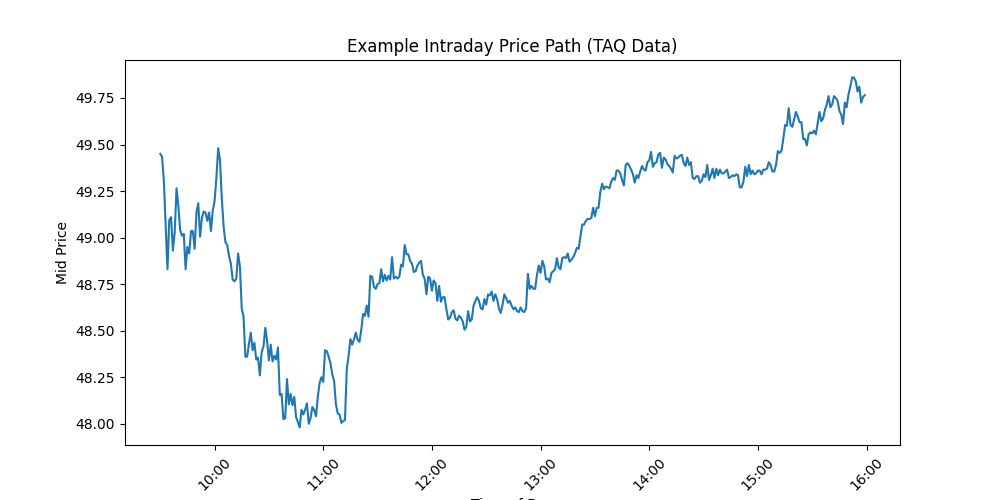
\includegraphics[width=0.8\textwidth]{../_output/taq_intraday_midprice_example.png}
\caption{Example intraday mid-price path constructed from TAQ minute-level quote data.}
\label{fig:taq_intraday_example}
\end{figure}

Figure~\ref{fig:ravenpack_news_flow} presents the number of RavenPack news events per day over the sample period. The figure illustrates that the arrival of firm-specific news varies substantially across days, reflecting periods of higher and lower information flow in financial markets.

\begin{figure}[H]
\centering
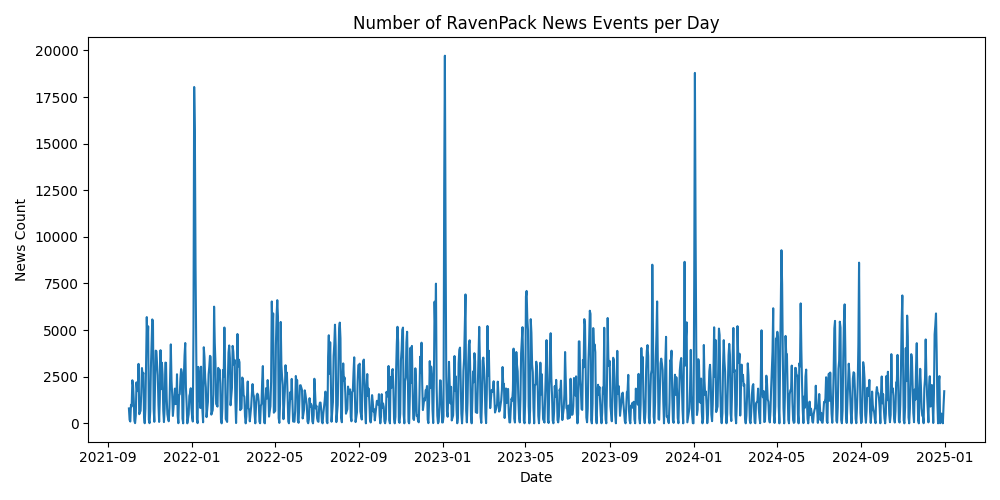
\includegraphics[width=0.8\textwidth]{../_output/ravenpack_news_per_day.png}
\caption{Daily number of RavenPack news events over the sample period.}
\label{fig:ravenpack_news_flow}
\end{figure}

Finally, Figure~\ref{fig:gpt_label_distribution} shows the distribution of sentiment labels generated by the language model. Each news headline is classified as positive (YES), negative (NO), or unknown (UNKNOWN). These classifications form the trading signals used to construct the long and short portfolios.

\begin{figure}[H]
\centering
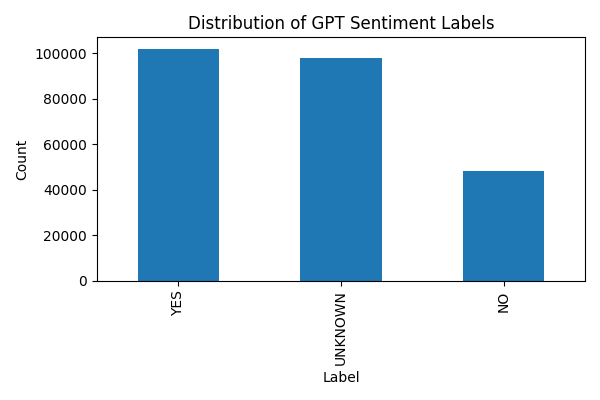
\includegraphics[width=0.6\textwidth]{../_output/gpt_label_distribution.png}
\caption{Distribution of sentiment labels generated by the language model.}
\label{fig:gpt_label_distribution}
\end{figure}

\section{Methodology}

The replication follows several main steps. First, news headlines are classified into sentiment categories using a language model. Headlines labeled as positive are interpreted as signals to take long positions, while headlines labeled as negative are interpreted as signals to take short positions.

Next, these labeled headlines are merged with stock return data. The timestamp of each news event is used to determine whether the information occurs during trading hours or outside trading hours. Based on this classification, returns are aligned with the appropriate trading window.

After the data are aligned, the strategy constructs daily long and short portfolios. The long portfolio consists of stocks associated with positive news, while the short portfolio consists of stocks associated with negative news. Portfolio returns are computed by averaging the event returns of the securities on each side of the strategy.

Finally, cumulative returns and summary performance statistics are computed to evaluate the effectiveness of the strategy.

\section{Results}

This section reports the main empirical outputs generated by the replication code.

\subsection{Performance Summary}

Table~\ref{tab:performance} reports summary statistics for the replicated trading strategy.

\begin{table}[H]
\centering
\footnotesize
\caption{Performance Summary of the Replicated Strategy}
\label{tab:performance}
\setlength{\tabcolsep}{4pt}
\renewcommand{\arraystretch}{1.1}
\resizebox{\textwidth}{!}{%
\begin{tabular}{lllrrrr}
 & \multicolumn{2}{r}{} & \multicolumn{2}{r}{Overnight News} & \multicolumn{2}{r}{Intraday News} \\
 & Portfolio Group & Metric & Initial Reaction & Drift & Initial Reaction & Drift \\
0 & Long-Short Portfolio & Hit Rate (%) & 96.23 & 54.97 & 88.94 & 50.16 \\
1 & Long-Short Portfolio & Mean Return (%) & 2.45 & 0.12 & 4.12 & 0.01 \\
2 & Long-Short Portfolio & Sharpe Ratio &  & 1.38 &  & 0.07 \\
3 & Long-Only Portfolio & Hit Rate (%) & 82.51 & 49.48 & 78.67 & 52.04 \\
4 & Long-Only Portfolio & Mean Return (%) & 0.89 & 0.00 & 1.61 & 0.10 \\
5 & Long-Only Portfolio & Sharpe Ratio &  & 0.04 &  & 0.96 \\
6 & Short-Only Portfolio & Hit Rate (%) & 85.09 & 53.61 & 80.80 & 50.93 \\
7 & Short-Only Portfolio & Mean Return (%) & 1.55 & 0.11 & 2.53 & -0.08 \\
8 & Short-Only Portfolio & Sharpe Ratio &  & 0.97 &  & -0.61 \\
9 &  & Firm-Day Observations & 61973.00 & 61973.00 & 13197.00 & 13197.00 \\
10 &  & Trading Days & 664.00 & 664.00 & 642.00 & 642.00 \\
\end{tabular}

}
\end{table}

The table summarizes key performance metrics for the strategy, including average returns and risk-adjusted measures. These statistics provide an overview of how profitable the trading strategy is over the sample period.

\subsection{Cumulative Returns}

Figure~\ref{fig:cumret} shows the cumulative return of the strategy over time.

\begin{figure}[H]
\centering
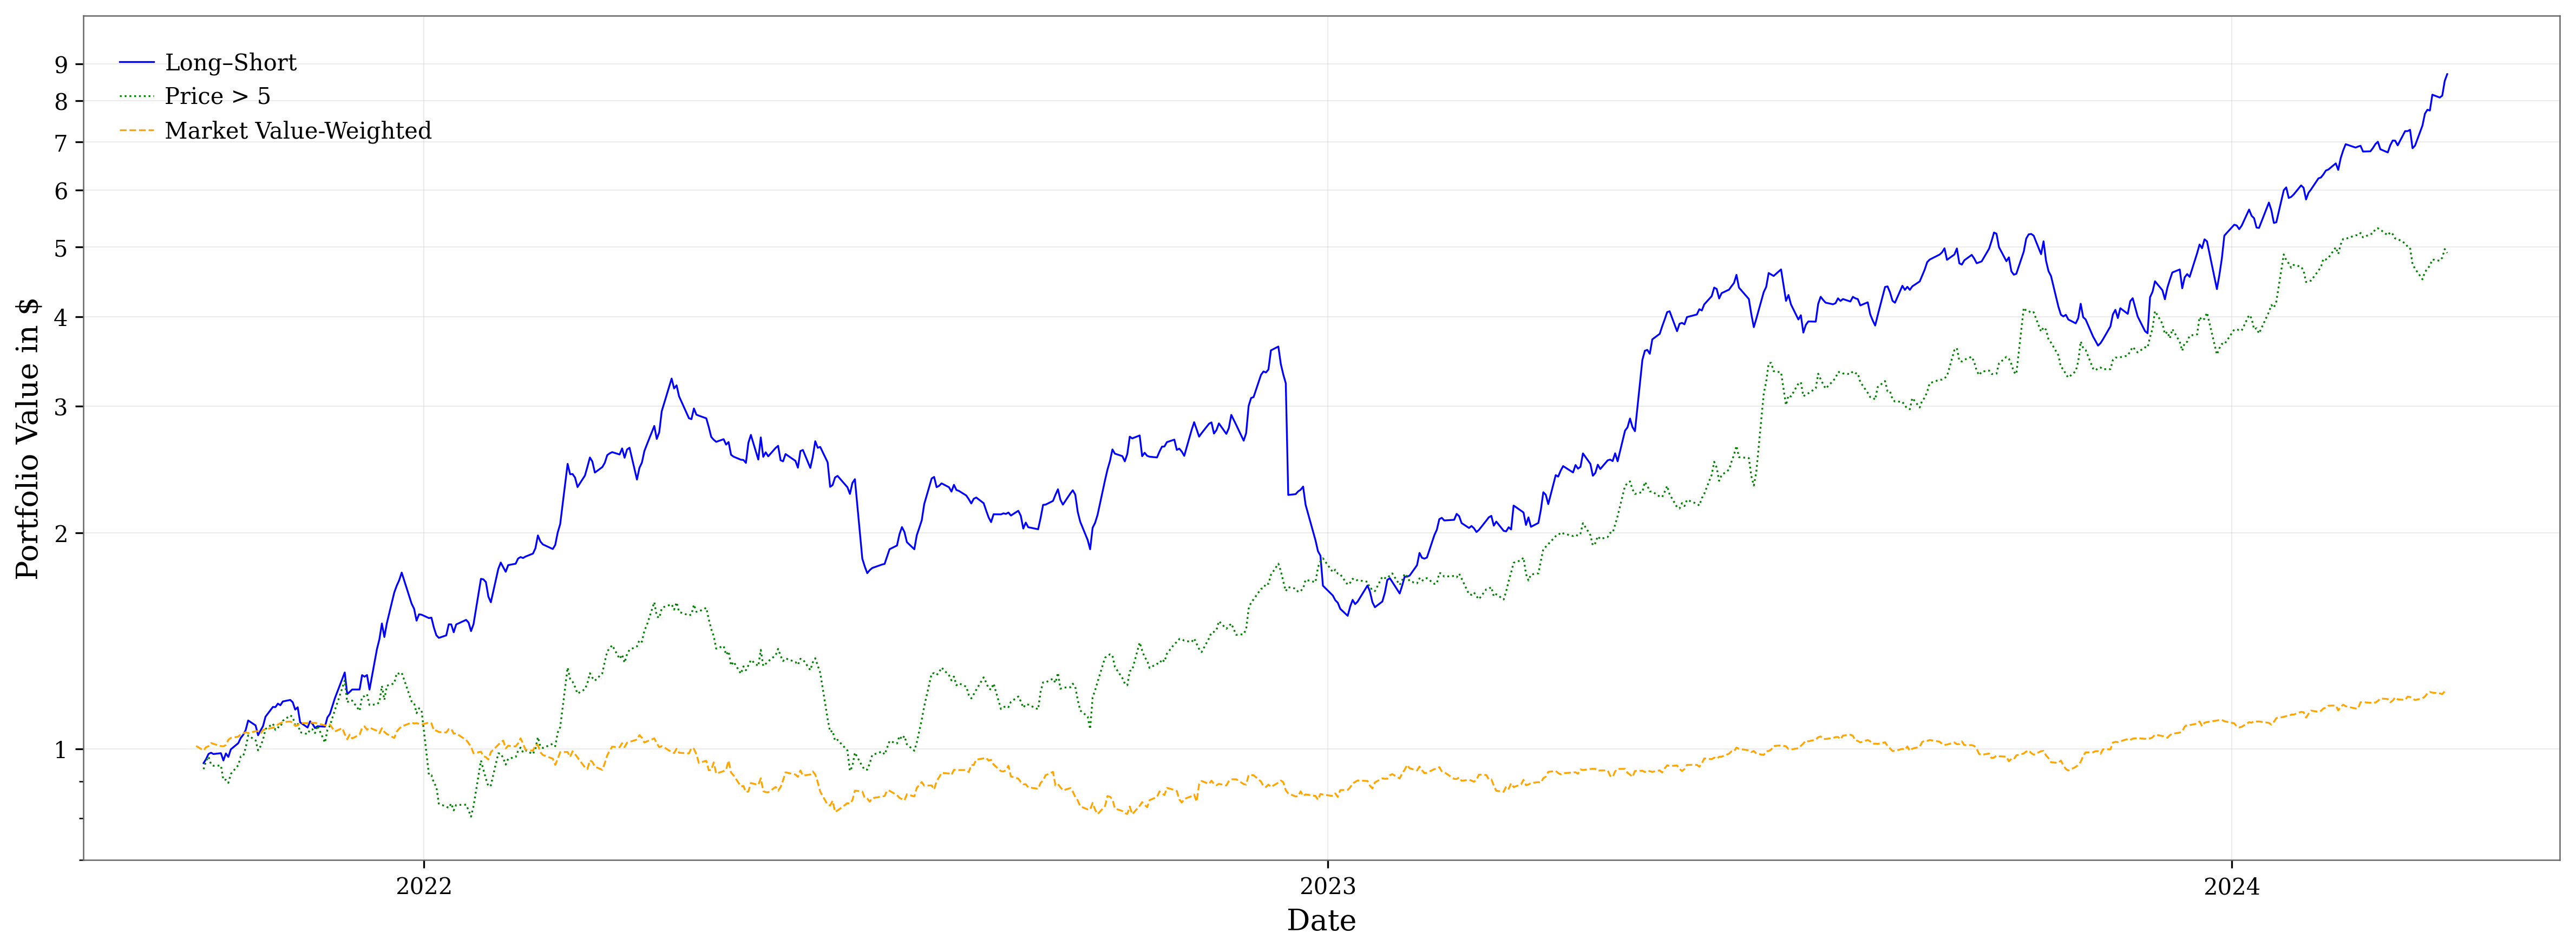
\includegraphics[width=1.1\textwidth]{../_output/cumulative_returns_paper_style.png}
\caption{Cumulative Returns of the Replicated Trading Strategy}
\label{fig:cumret}
\end{figure}

The cumulative return plot provides a visual representation of how the strategy performs through time. It illustrates whether the trading signals generate consistent performance or whether returns are concentrated in particular periods.

\section{Discussion}

The replication was successful in constructing a full empirical pipeline that integrates textual news data with financial market data. One of the main successes of the project was the ability to combine multiple datasets and transform them into a coherent trading framework. The resulting outputs, including performance tables and cumulative return charts, provide a clear view of the behavior of the strategy.

However, the replication also encountered several challenges. One challenge was aligning the timing of news events with tradable return windows. Small errors in timestamp alignment can significantly affect measured returns. Another challenge was handling cases where multiple news headlines occurred for the same firm on the same day. Aggregating these signals required careful design decisions.

Additionally, the profitability of the strategy can be sensitive to filtering rules, such as excluding low-priced stocks or requiring a minimum number of securities on each side of the portfolio. These implementation choices can lead to differences between the replicated results and the original study.

Despite these challenges, the replication demonstrates that sentiment-based signals extracted from news headlines can be incorporated into systematic trading strategies. The results suggest that textual information may contain economically meaningful signals for financial markets.

\section{Conclusion}

This project replicated a news-based trading strategy that uses sentiment-labeled headlines to construct long and short portfolios. By combining news data, sentiment classification, and stock return data, the project created a complete framework for evaluating the predictive value of textual information.

The replication successfully produced performance tables and cumulative return charts that summarize the behavior of the strategy. While the results depend on implementation details and data alignment, the overall framework demonstrates how machine learning methods and textual data can be integrated into quantitative trading research.

Future work could extend the analysis by incorporating additional sentiment features, improving the classification model, or testing the strategy across different market environments.

\end{document}